


\begin{table*}[ht]
	\caption{関数に必要な情報とその対応表} \label{}
	\textit{注: $\circ$は必須引数,$\triangle$はオプショナル引数を示す} \label{tab:my_label}
	\centering
	\scalebox{0.5}{
		\begin{tabular}{|c|c|c|c|c|c|c|c|c|c|c|c|c|c|} 

			\hline
			                   & 処理名& \multicolumn{4}{c|}{センサ情報}   & \multicolumn{3}{c|}{環境情報}    & \multicolumn{4}{c|}{その他}                                                                                                                                                                                                                                                                                                                                 \\ \hline
			                   &                                                                     &                              &                              &                              & \multicolumn{1}{c|}{BLEビーコン} &                              &  \multicolumn{2}{c|}{BLEビーコン} & \multicolumn{2}{c|}{正解初期}        & \multicolumn{2}{c|}{正解補正}                                                 \\ \cline{6-6} \cline{8-8} \cline{9-9} \cline{10-10}\cline{11-12}\cline{13-13}
			                   &                                                                     & 加速度                          & 角速度                          & 角度                           & 電波強度・AP情報                    & フロアマップ                                                                                                                                   & 基地局位置                        & FP                               & 座標                               & 姿勢 & 座標                           & 姿勢 \\ \hline
			estimate\_trajectory  &    基本PDR                                                           & \multicolumn{1}{c|}{$\circ$} & \multicolumn{1}{c|}{$\circ$} &                              &                                                            &                                                                                                               &                              &                                  & \multicolumn{1}{c|}{$\triangle$} &    &                              &    \\ \hline
			convert\_to\_angle\_from\_gyro                                       & 角速度から角度推定          &                              & \multicolumn{1}{c|}{$\circ$} &                              &                              &                                                                                                                                             &                              &                                  &                                  &    &                              &    \\ \hline
			remove\_drift\_in\_angle                                           & ドリフト補正              & \multicolumn{1}{c|}{$\circ$} &                              & \multicolumn{1}{c|}{$\circ$} &                              &                                                                                                                                             &                              &                                  & \multicolumn{1}{c|}{$\circ$}     &    & \multicolumn{1}{c|}{$\circ$} &    \\ \hline
			rotate\_trajectory\_to\_optimal\_alignment\_using\_map             &  初期進行方向補正 歩行可能領域マップ & \multicolumn{1}{c|}{$\circ$} &                              & \multicolumn{1}{c|}{$\circ$} &                              & \multicolumn{1}{c|}{$\circ$}                                                                                                                &                              &                                  & \multicolumn{1}{c|}{$\triangle$} &    &                              &    \\ \hline
			rotate\_trajectory\_to\_optimal\_alignment\_using\_ble             &  初期進行方向補正 BLE       & \multicolumn{1}{c|}{$\circ$} &                              & \multicolumn{1}{c|}{$\circ$} & \multicolumn{1}{c|}{$\circ$} &                                                                                                                                             & \multicolumn{1}{c|}{$\circ$} &                                  & \multicolumn{1}{c|}{$\triangle$} &    &                              &    \\ \hline
			move\_unwalkable\_points\_to\_walkable                             &  マップマッチング補正        & \multicolumn{1}{c|}{$\circ$} &                              & \multicolumn{1}{c|}{$\circ$} &                              & \multicolumn{1}{c|}{$\circ$}                                                                                                                &                              &                                  & \multicolumn{1}{c|}{$\triangle$} &    &                              &    \\ \hline
	rotate\_trajectory\_to\_optimal\_alignment\_using\_ble\_fingerprint
		& 	初期進行方向補正 BLE FP    		                   & \multicolumn{1}{c|}{$\circ$}                                        &                              & \multicolumn{1}{c|}{$\circ$} &                                                            &                              &                                                                                                               & \multicolumn{1}{c|}{$\circ$} & \multicolumn{1}{c|}{$\triangle$} &                                  &    &                                   \\ \hline
		\end{tabular}
	}
\end{table*}




関数に必要な引数の情報をいくつかの種類に分類し,それを各関数に対応づけたものを表1に示す.
詳しい関数の説明や内部実装については後述する.
引数の情報は大きく分けてセンサ情報,環境情報,その他の3つに分類される.
センサ情報はスマートフォンから得られる加速度,角速度,BLEビーコンの電波情報などが含まれる.
環境情報はフロアマップ,フロアマップにおける各BLEビーコンの配置情報などが含まれる.
これらの環境情報は全てセンサデータが与えられる前に得られる情報である.
その他はセンシング中,またはセンシング前に得られる情報であり,初期位置,終了位置などの情報が該当する.

本ライブラリの実装にはプログラミング言語PythonとそのライブラリであるPandasを主に使用した.
Pythonには科学技術関連ライブラリが豊富に存在し,Numpy,Pandas,Scikit-learn,Matplotlibなどデータ分析や機械学習を支援する強力なライブラリがある.
特にPandasライブラリはデータ解析を容易にする多くの機能を提供している.
Pandasはデータフレーム(以下,DF)と呼ばれるデータ構造を提供し,
DFは表形式のデータを扱うための強力なツールであり,
行と列から構成される2次元のデータ構造である.
PandasはDFの操作を容易にする機能を提供し,
これにより大量のセンサデータを効率的に操作・分析できる.
これは本ライブラリ内部処理において必要なデータの読み込み,集約,フィルタリングといった操作に適している.
そのため本ライブラリの引数や内部処理のデータ構造にもPandasのDFが使用されている.

\begin{table}[ht]
	\caption{加速度 DF}
	\centering
	\begin{tabular}{lll}
		\toprule
		カラム名 & 単位        & データ型  \\
		\midrule
		ts   & s (秒)     & float \\
		x    & m/s\(^2\) & float \\
		y    & m/s\(^2\) & float \\
		z    & m/s\(^2\) & float \\
		\bottomrule
	\end{tabular}
\end{table}

\begin{table}[ht]
	\caption{角速度 DF}
	\centering
	\begin{tabular}{lll}
		\toprule
		カラム名 & 単位             & データ型  \\
		\midrule
		ts   & s (秒)          & float \\
		x    & rad/s (ラジアン/秒) & float \\
		y    & rad/s (ラジアン/秒) & float \\
		z    & rad/s (ラジアン/秒) & float \\
		\bottomrule
	\end{tabular}
\end{table}


加速度DF,角速度DFのデータフレームのカラム名とデータ型を表2,表3に示す.
オプショナル引数として正解初期座標(ground\_truth\_first\_point)を与えられる.
正解初期座標は辞書型で表4に示す.
戻り値は時間経過に伴う2次元座標のDF(以下,座標DF)と角度DFであり,それぞれのカラム名とデータ型を表5,表6に示す.
戻り値として角度DFを返しているのは各補正関数が角度DFを引数として受け取る設計なためである.
各補正関数は内部で角度DFを使用し処理を行っており,角速度DFを引数として受け取る場合に比べ,積分処理を省略できる利点がある.

\begin{table}[ht]
	\caption{正解初期座標 DICT}
	\centering
	\label{tab:first-coord-dict}
	\begin{tabular}{lll}
		\hline
		      & {データ型}         & {説明}          \\ \hline
		key   & \texttt{str}   & xまたはy         \\ \hline
		value & \texttt{float} & \makecell{座標} \\ \hline
	\end{tabular}
\end{table}


\begin{table}[ht]
  \caption{時間経過に伴う2次元座標DF(座標DF)}
	\centering
	\begin{tabular}{lll}
		\toprule
		カラム名 & 単位      & データ型  \\
		\midrule
		ts   & s (秒)   & float \\
		x    & m(メートル) & float \\
		y    & m(メートル) & float \\
		\bottomrule
	\end{tabular}
\end{table}


\begin{table}[ht]
  \caption{角度 DF}
	\centering
	\begin{tabular}{lll}
		\toprule
		カラム名 & 単位         & データ型  \\
		\midrule
		ts   & s (秒)      & float \\
		x    & rad (ラジアン) & float \\
		y    & rad (ラジアン) & float \\
		z    & rad (ラジアン) & float \\
		\bottomrule
	\end{tabular}
\end{table}


本ライブラリの実装では歩幅や歩行タイミングの正確な推定を行わない.
歩幅の推定を行っている研究は多くある.
機会学習を用いた研究\cite{stride-length-auto-learning},
多変量解析を用いた研究\cite{stride-length-multi},
超音波センサーガジェットを用いた研究\cite{stride-length-ultrasonic}などがある.
本関数の内部処理では歩幅の値は固定値として扱っている.
本来であれば歩幅は身長,性別,年齢などの複数の要素によって動的に変化するため
固定値なのはありえず,先ほど挙げた研究のように歩幅を推定する必要がある.
しかし本ライブラリの目的は正確な歩幅を用いたPDRによる位置推定ではない.
そのため歩幅の推定は行わず固定値として扱う.
また同様の理由で歩行タイミングの検出も正確には行わず,加速度の値が特定の閾値を超えた時を
歩行タイミングとして扱っている.

\begin{figure}[ht]
	\centering
	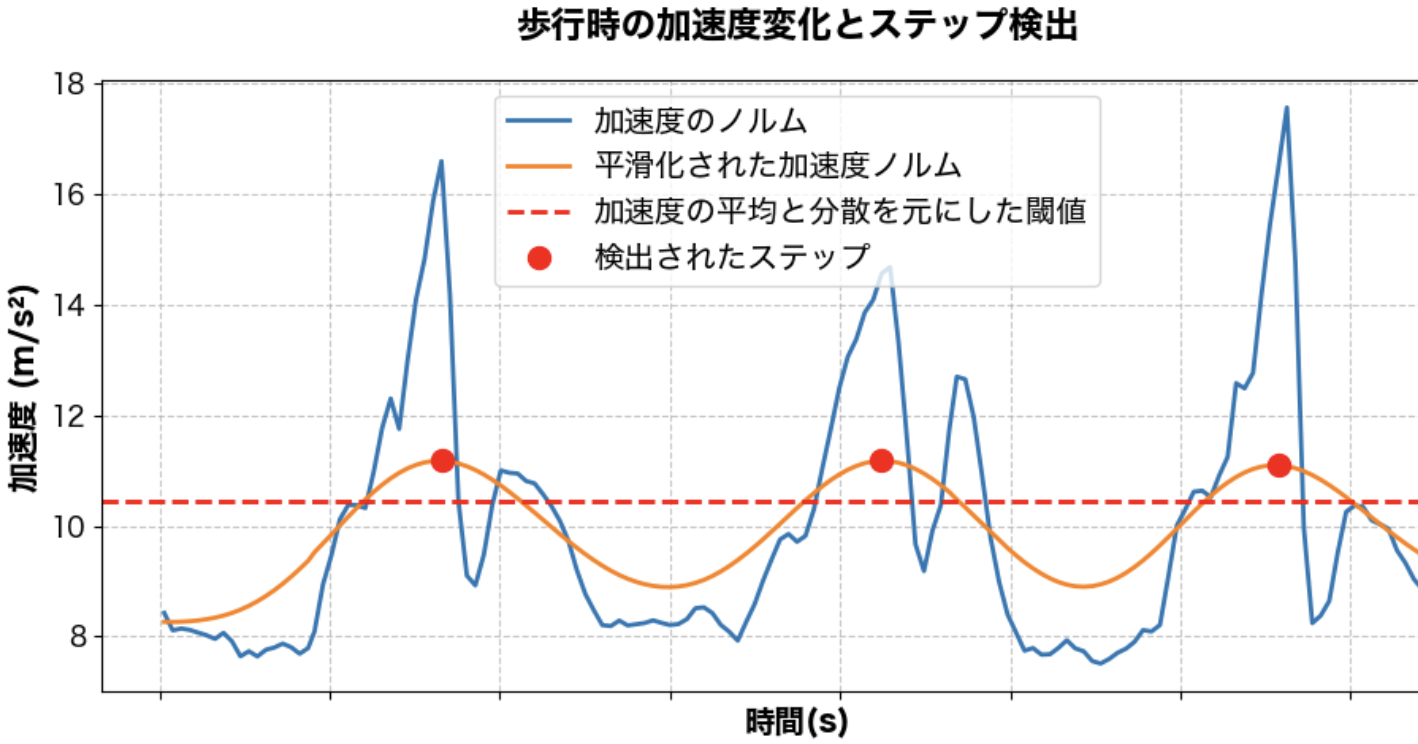
\includegraphics[width=130mm]{image/step_detect.jpg}
	\caption{加速度を利用したステップ検出}    \label{fig:step_detect}
\end{figure}


\begin{figure}[ht]
	\centering
	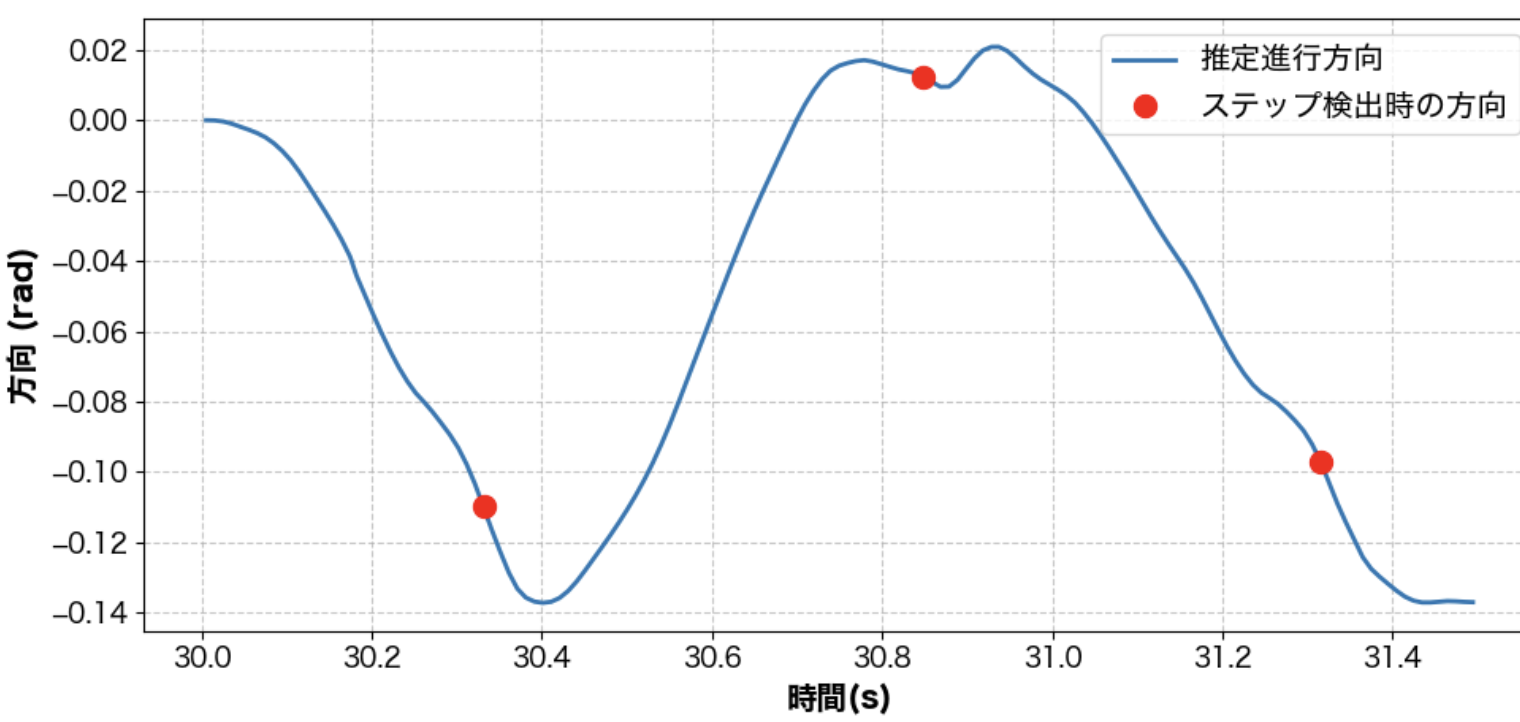
\includegraphics[width=130mm]{image/step_timing_angle.jpg}
	\caption{推定進行方向の変化}    \label{fig:step_timing}
\end{figure}


xDR Challenge 2023で与えられたトレーニングデータの
一部に対してライブラリを用いて位置推定を行いそれが
どのように変更されるのか図を用いて示していく.
図\ref{fig:pdr}にListing\ref{lst:pdr-trajectory}を用いてPDRによる位置推定を行った結果を示す.
この図は2次元座標上に推定軌跡を表し,カラーバーが経過時間を表している.
LiDARで取得した座標を基に出力された軌跡を図\ref{fig:gt-trajectory}に示す.
これを本論では正解軌跡とする.
図\ref{fig:pdr}と図\ref*{fig:gt-trajectory}を比較するとPDRによる軌跡は正解軌跡と比べて大きくずれているのがわかる.
PDR特有の解決すべきものとして
軌跡そのものの形状を正解軌跡に近づける問題と絶対位置との関連付けの問題がある.
本ライブラリを用いてこれらの問題を解消し正解軌跡に近づけていく.
Listing\ref{lst:pdr-trajectory}に示される関数に正解初期座標を
与えたのが図\ref{fig:pdr-move}である.
予め正解座標が判明している場合はPDRによる軌跡の初期位置を補正できる.



% 文書内
\begin{lstlisting}[caption={基本PDR}, label=lst:pdr-trajectory,float =h]
Axis2D = Literal["x", "y"]
def estimate_trajectory(
    acc_df: pd.DataFrame,
    gyro_df: pd.DataFrame,
    *,
    ground_truth_first_point: dict[Axis2D, float] | None = None,
) -> tuple[pd.DataFrame, pd.DataFrame]:
\end{lstlisting}

\begin{figure}[ht]
	\centering
	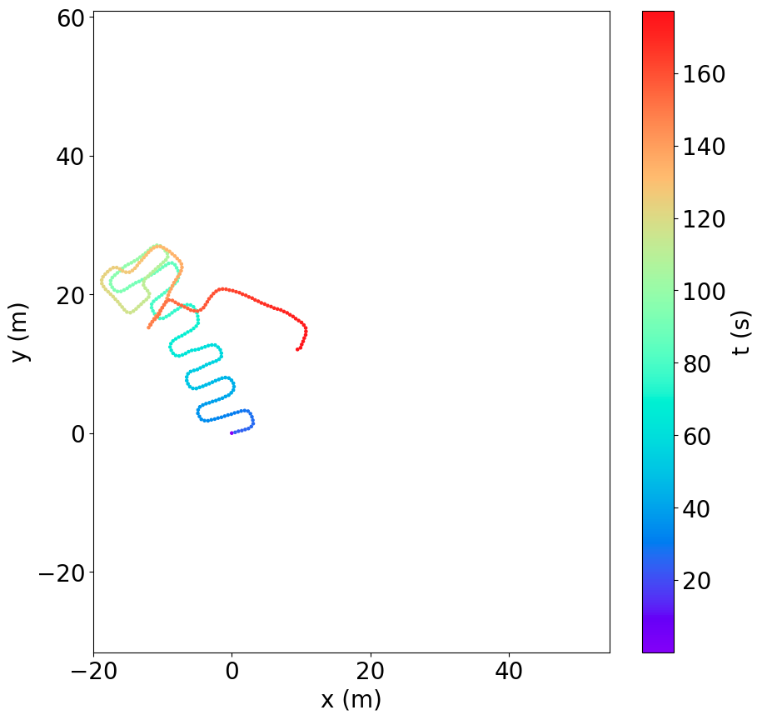
\includegraphics[width=80mm]{image/pdr.jpg}
	\caption{基本PDRの軌跡}    \label{fig:pdr}
\end{figure}

\begin{figure}[ht]
	\centering
	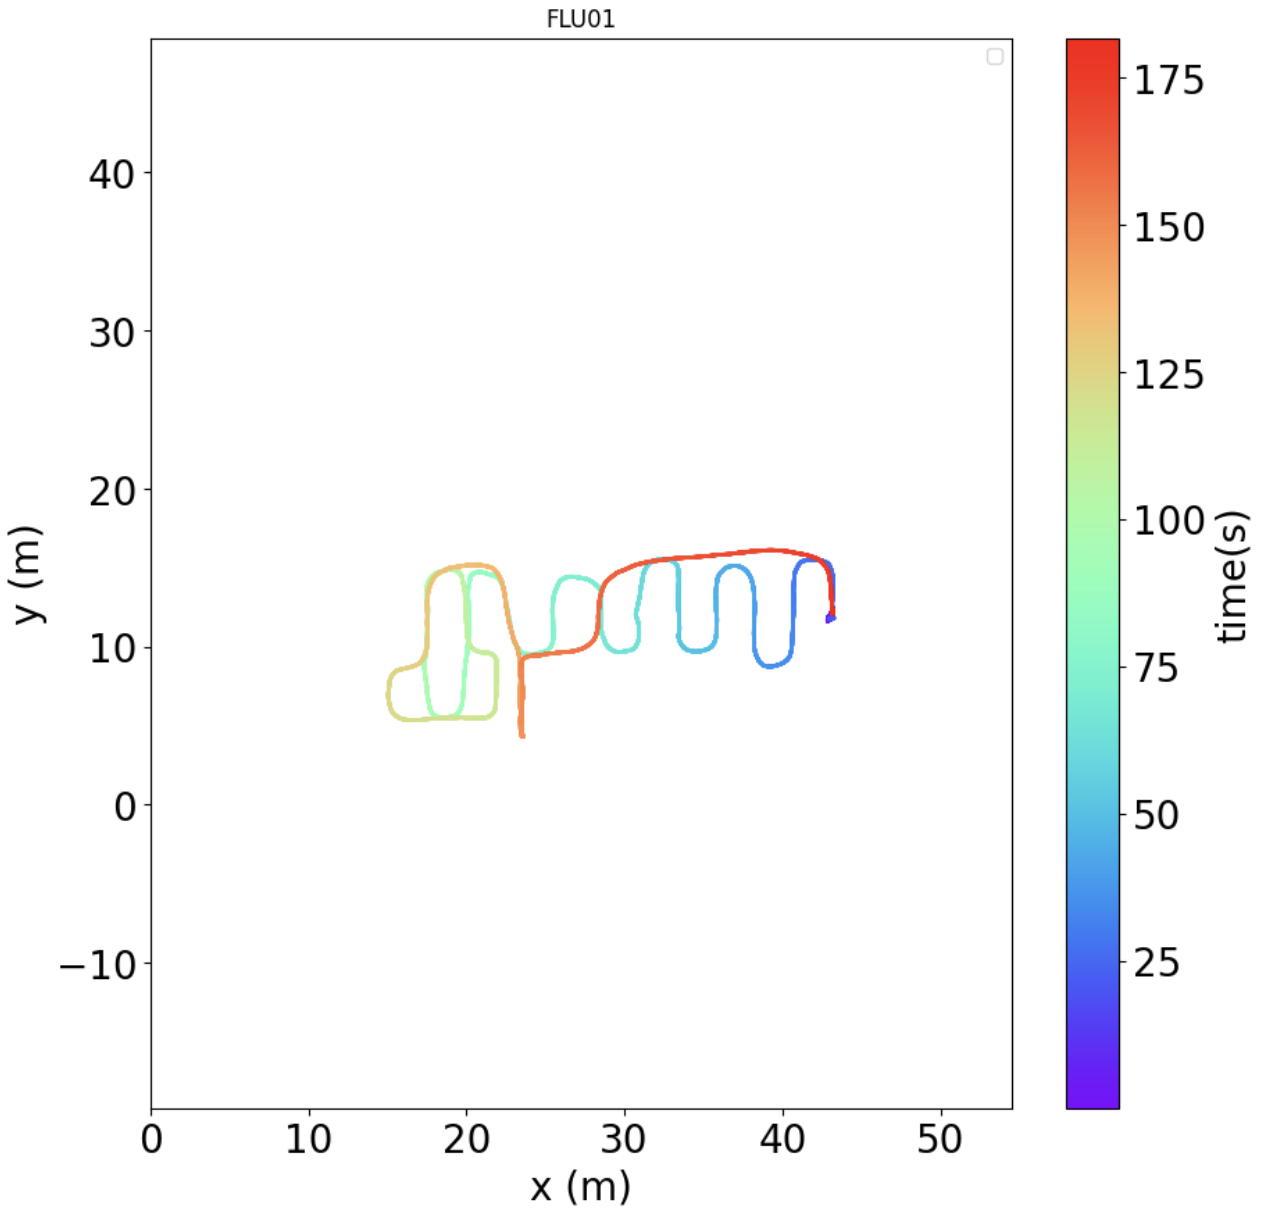
\includegraphics[width=80mm]{image/gt2.jpg}
	\caption{正解軌跡}    \label{fig:gt-trajectory}
\end{figure}

\begin{figure}[ht]
	\centering
	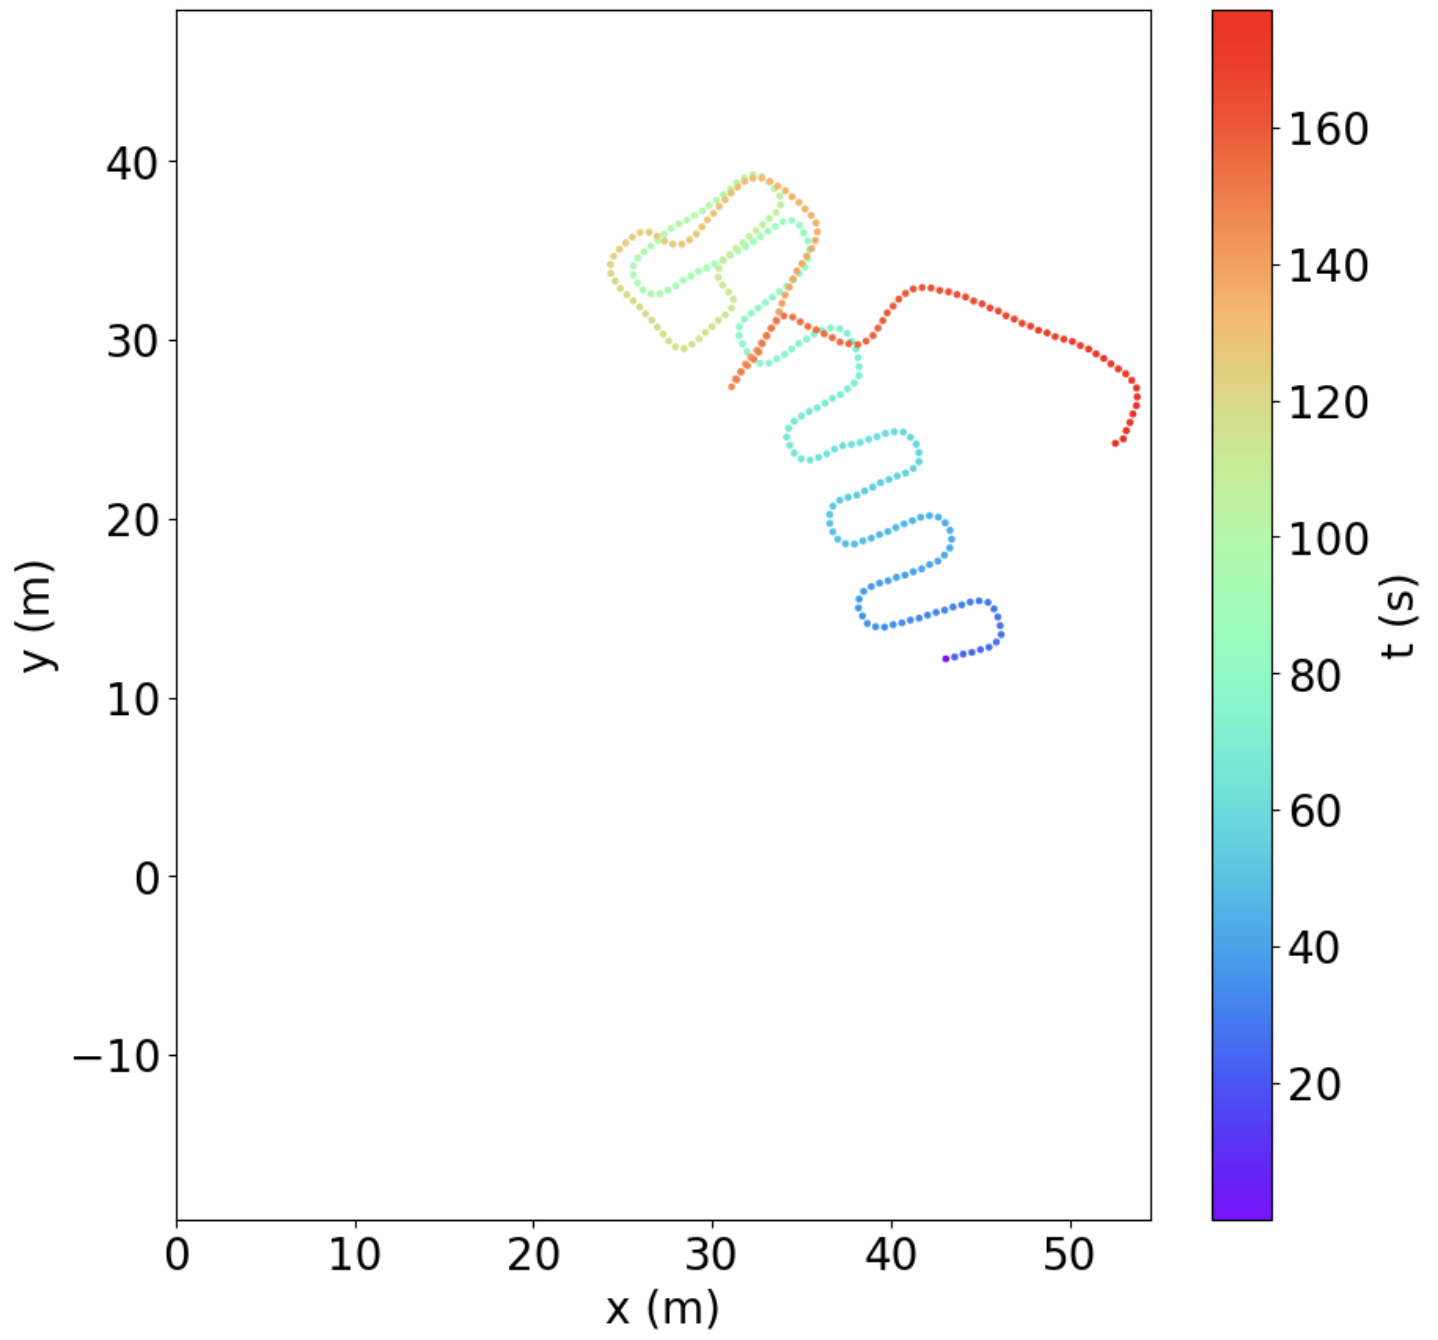
\includegraphics[width=80mm]{image/pdr-move.jpg}
	\caption{正解初期座標が存在}    \label{fig:pdr-move}
\end{figure}





